%% This is file `elsarticle-template-1-num.tex',
%%
%% Copyright 2009 Elsevier Ltd
%%
%% This file is part of the 'Elsarticle Bundle'.
%% ---------------------------------------------
%%
%% It may be distributed under the conditions of the LaTeX Project Public
%% License, either version 1.2 of this license or (at your option) any
%% later version.  The latest version of this license is in
%%    http://www.latex-project.org/lppl.txt
%% and version 1.2 or later is part of all distributions of LaTeX
%% version 1999/12/01 or later.
%%
%% The list of all files belonging to the 'Elsarticle Bundle' is
%% given in the file `manifest.txt'.
%%
%% Template article for Elsevier's document class `elsarticle'
%% with numbered style bibliographic references
%%
%% $Id: elsarticle-template-1-num.tex 149 2009-10-08 05:01:15Z rishi $
%% $URL: http://lenova.river-valley.com/svn/elsbst/trunk/elsarticle-template-1-num.tex $
%%
% \documentclass[preprint,12pt]{elsarticle}

%% Use the option review to obtain double line spacing
%% \documentclass[preprint,review,12pt]{elsarticle}

%% Use the options 1p,twocolumn; 3p; 3p,twocolumn; 5p; or 5p,twocolumn
%% for a journal layout:
%% \documentclass[final,1p,times]{elsarticle}
%% \documentclass[final,1p,times,twocolumn]{elsarticle}
%  \documentclass[final,3p,times]{elsarticle}
 \documentclass[final,3p,times,twocolumn]{elsarticle}
%% \documentclass[final,5p,times]{elsarticle}
%% \documentclass[final,5p,times,twocolumn]{elsarticle}

%% if you use PostScript figures in your article
%% use the graphics package for simple commands
%% \usepackage{graphics}
%% or use the graphicx package for more complicated commands
%% \usepackage{graphicx}
%% or use the epsfig package if you prefer to use the old commands
%% \usepackage{epsfig}

\usepackage[utf8]{inputenc} 
%% The amssymb package provides various useful mathematical symbols
\usepackage{amssymb}
\usepackage{hyperref}
\usepackage{graphicx}
\usepackage{subcaption}
\usepackage{lscape}
\usepackage{amsmath}
\usepackage{multirow}
% if you have landscape tables
\usepackage[figuresright]{rotating}
\usepackage{lineno}
\usepackage{algorithm} 
\usepackage{algpseudocode} 
\usepackage{comment}
\usepackage{lineno}

\usepackage{natbib}
\bibliographystyle{abbrvnat}
\setcitestyle{authoryear,open={(},close={)},citesep={;}} 

\usepackage{calc}
\setlength{\footskip}{\paperheight
  -(1in+\voffset+\topmargin+\headheight+\headsep+\textheight)
  -0.95in}

% for SVG figures
\usepackage{svg}

% For using LuaLaTeX or XeLaTeX compilers instead of pdflatex (memory limit)
\usepackage{fontspec} 
\setmainfont{Times New Roman}

\usepackage{titlesec}
\titleformat{\section}{\normalfont\bfseries}{\thesection}{1em}{}
\titleformat{\subsection}{\normalfont\itshape}{\thesubsection}{1em}{}


\begin{document}

\begin{frontmatter}

% \title{Automated Identification of Invasive Aquatic Plants Using Deep Neural Networks on Controlled Image Datasets}
\title{Improving Out-of-Distribution Aquatic Plant Classification from Limited Controlled Training Data Using Confidence-Aware Re-Evaluation}

\author[label1]{Aaryan Panigrahi}
\author[label1]{Fengying Dang}


\address{Fengying Dang (fdang1@mtu.edu) is the corresponding author}
\address[label1]{Department of Electrical and Computer Engineering, Michigan Technological University, Houghton, MI 49931, USA}


\begin{abstract}
 % Focus on why the problem is hard - limited data and complex env - current limitations
Aquatic invasive species (AIS) threaten the resilience of fisheries and aquaculture systems, causing severe ecological damage and economic losses. Accurate early identification is necessary to manage these species. However, collecting high-quality images in underwater environments is difficult and expensive, resulting in limited available data. Consequently, computer vision models trained on small laboratory datasets often fail to generalize to the visual variations found in natural settings. To address this limitation, this study introduces the `You Need To Look Twice' (YNLT) module. Inspired by the human behavior of closely re-examining uncertain details, this confidence-aware module identifies ambiguous image regions and re-evaluates them at higher resolutions. The YNLT module is supported by a ConvNeXt-V2 backbone and a Gated Attention classification head to extract relevant plant features while filtering out background artifacts. The method was evaluated using a dataset of 225 plant images captured in a controlled laboratory. To test generalization to out-of-distribution environments, an additional dataset of 33 crowd-sourced images showing plants in field settings was used. The proposed approach increases classification accuracy from a baseline of 84.78\% to 93.48\% on the laboratory test set. Furthermore, it improves accuracy on the out-of-distribution crowd-sourced images from 47.06\% to 64.71\%. These results indicate that models trained on limited laboratory images can learn to identify invasive plants in more complex environments, providing a practical tool to support fisheries management and prevent ecological damage...
\end{abstract}

\begin{keyword}
Aquatic invasive species \sep Computer vision \sep precision agriculture \sep Domain generalization \sep Environmental monitoring
\end{keyword}

\end{frontmatter}

%%%%%%%%%%%%%%%%%%%%%%%%%%%%%%%%%%%%%%%%%%%%%%%%%%%%%%%%%%%%%%%%%%%%%%%%%%%%%%%%%%%%%%%%%%%%%%%%%%%%%%%%%%%%%%%%%%%%%%%%%%%%%%%%%%%%%%
%% main text
\section{Introduction}
\label{sec:intro}

%% Structure
% 1. Opening Motivation with broad problems in the field
% 2. Specific/Core problem we will address
% 3. Approaches to the problem across all the different fields
% 4. Why Computer Vision and Deep learning is promising
% 5. Specific research gaps @ deep learning for this problem
% 6. Our objectives and contributions

%% 1. Opening Motivation with broad problems in the field

Invasive species significantly threaten biosecurity and harm the economy, natural and cultural resources, infrastructure, agricultural production, and human health~\cite{tasker2024nuanced, macedo2024economic, shen2024typical}. Annual economic damages and control costs of invasive species around the world are estimated to exceed several trillion dollars~\cite{vaissiere2022nature, macedo2024economic, cuthbert2021global}. Recent estimates suggest that exotic invasive species cost the American economy approximately \$138 billion annually~\cite{pimentel2000environmental, lovell2006economic, warziniack2021economics, macedo2024economic}. The majority of these costs are related to freshwater invasive plants, with most costs incurred by submerged (59\%) and floating (34\%) invasive plants~\cite{macedo2024economic}.


%% ??Need to be rewrite??
Aquatic invasive plants pose significant threats to both fish farms and natural fisheries by disrupting ecological balance and increasing operational burdens. Dense growth of invasive macrophytes such as Hydrilla, Eichhornia crassipes (water hyacinth), and Salvinia molesta can form thick surface mats that block sunlight penetration, leading to oxygen depletion in the water column—especially at night—causing fish stress or mass mortality. These plants also physically alter aquatic habitats, reducing spawning and nursery areas critical for fish reproduction. In cage and pond-based aquaculture systems, they can interfere with feeding behavior by clogging gills or obstructing access to feed zones, resulting in reduced growth rates. Moreover, stagnant water conditions beneath dense vegetation can foster the spread of parasites and pathogens, elevating disease risk and mortality. From an operational perspective, invasive plants increase maintenance costs by clogging nets, pumps, aerators, and water intake systems, and they can hinder navigation and access to cages or harvest zones. The cumulative effect of these impacts can severely reduce fish production and drive up labor and management costs, posing a major threat to the sustainability and profitability of aquaculture operations.

% Unlike chemical pollutants, invasive species can reproduce and spread, making the problem worse over time. Once established, they disrupt native ecosystems, and eradicating them is often difficult and costly. With more trade and travel, biological invasions are likely to increase, highlighting the growing importance of research on invasive aquatic species~\cite{motitsoe2022invasive}.

% 2. Specific/Core problem we will address
The economic and ecological impact of aquatic invasive species discussed above underline the importance of being able to accurately identify them at scale. Existing AIS identification approaches include field-based morphological identification~\cite{dehez2023investigation}, molecular methods~\cite{angles2019detection, ghahramanzadeh2013efficient, scriver2015development}, remote sensing~\cite{brooks2019implementing, unitis2018remote, jochems4883509active}, and image-based computer vision~\cite{wang2026realtime}.

% Currently, there are four major approaches to this problem: (1) Human eye ~\cite{dehez2023investigation}; (2) DNA analysis~\cite{angles2019detection, ghahramanzadeh2013efficient, scriver2015development}; (3) Remote sensing ~\cite{brooks2019implementing, unitis2018remote, jochems4883509active}; (4) Computer Vision ~\cite{wang2026realtime}. 

Human eye-based classification from botanical knowledge or experience is the most common method in use today, as it doesn't require any equipment or resources. But it is time-consuming, and accuracy varies with expertise. DNA-based methods typically require specialized equipment, expertise, and resources for sample collection, DNA extraction, amplification, sequencing, and analysis ~\cite{angles2019detection, ghahramanzadeh2013efficient}. Both of these methods are impractical at scale. Remote sensing can operate at a larger scale, but has limitations in detail, accuracy in complex environments, and effectiveness with submerged or obscured vegetation~\cite{brooks2019implementing, unitis2018remote, jochems4883509active}. 


% 4. Why Computer Vision and Deep learning are promising
Computer vision methods are a promising alternative, that rely only on standard images captured by any camera. A computer vision solution could potentially be deployed on devices ranging from smartphones to underwater robots, enabling efficient and accurate identification of AIS at a large scale. They are cost-effective and accessible as they can be deployed on any device with a camera. Their ability to provide real-time decisions makes them useful and efficient at scale. 

Early attempts to apply computer vision to species identification relied heavily on feature engineering. Handcrafted features such as contours for shapes, Fourier descriptors for texture, and color histograms were extracted, and machine learning classifiers such as k-NNs, SVMs, and random forests were used to make decisions based on the extracted features. While these methods work well in simple, controlled conditions, they often fail to generalize to real-world environments due to variability such as background, lighting, scale, noise, etc.

The emergence of deep learning in recent times has shifted the paradigm from careful feature engineering to automated feature learning from more available data. Convolutional Neural Networks (CNNs) have been shown to be effective in several domains such as medical imaging, autonomous driving, and wildlife monitoring, where accurate recognition under challenging conditions is critical. The identification of AIS also faces many of the same challenges and is well-positioned to benefit from these advancements.

A substantial body of prior work has explored the use of convolutional neural networks (CNNs) for underwater plant classification. In particular, studies built on the DeepSeaGrass dataset have demonstrated that CNN-based architectures can effectively extract discriminative features from underwater optical imagery and achieve strong classification performance \cite{DeepSeaGrass1, Nawaz2025Seagrass}. These results, along with related efforts \cite{Paul2023LWDS, baos_cnn}, establish CNNs as a viable approach for recognizing aquatic flora in controlled or well-curated datasets.

However, these approaches exhibit important limitations when applied to freshwater ecosystems such as the Great Lakes of Michigan. First, many existing datasets, including DeepSeaGrass, involve visually distinct classes (e.g., different seagrass species), whereas freshwater environments often require fine-grained classification between morphologically similar invasive and native species. This significantly increases the difficulty of the task. Second, high-performing CNN-based methods typically rely on large-scale, well-labeled datasets and substantial computational resources \cite{baos_cnn}, conditions that are rarely met in aquatic monitoring applications where data collection is expensive and logistically constrained.

To mitigate data scarcity, prior work has explored transfer learning and classical machine learning approaches. For example, a hierarchical support vector machine (SVM) framework has been applied to kelp classification tasks, demonstrating that leveraging pre-trained features can improve performance under limited data regimes \cite{Kelps_SVMs}. While effective to a degree, such methods are inherently limited in their ability to model complex, high-dimensional visual patterns compared to modern deep learning architectures. This limitation becomes particularly pronounced in scenarios requiring discrimination between visually similar species under varying environmental conditions.

These challenges highlight a gap in existing approaches: there is a need for models that can both learn effectively from small, controlled datasets and generalize to out-of-distribution conditions encountered in natural environments. In this work, we focus on the classification of aquatic plant species in Michigan water bodies, with the goal of distinguishing invasive from native species. Due to the difficulty of acquiring high-quality underwater imagery, the available training data is limited and primarily collected in laboratory settings. Consequently, the model must not only achieve high accuracy on in-distribution data, but also maintain robustness when applied to field images exhibiting variations in lighting, turbidity, and background complexity.

In addition, the cost of different types of errors is asymmetric. Misclassifying an invasive species as native can lead to delayed intervention and significant ecological damage, whereas the reverse error is comparatively less critical. Therefore, beyond overall accuracy, the model should be designed to reduce false negatives for invasive species, ensuring more reliable detection in real-world deployment.

% 6. Our objectives and contributions
    % Image Classification
    % Generalization to different conditions
    % Minimize False Negatives



Our main contributions are as follows:

\begin{enumerate}
\item Computer Vision Models trained on this small dataset that generalize to images of the same plants in various settings
\item A novel confidence-aware ensemble based module called `You Need to Look Twice' (YNLT) that reduces False Negative predictions.
\item A parameter efficient `Gated Attention' classification head architecture to effectively generalize to out of domain data. 
\end{enumerate}

The remainder of the paper is organized as follows. The materials and methods for developing this paper are presented in Section \ref{sec:materials_methods}.  Experimental results and analysis are described in Section \ref{sec:results}. Conclusion remarks are drawn in Section \ref{sec:conclu}.


\section{Materials and Methods}
\label{sec:materials_methods}

\subsection{Study area}
\label{subsec:study_area}

The geographic focus of this study is the state of Michigan, which encompasses portions of four Great Lakes (Lake Superior, Lake Michigan, Lake Huron, and Lake Erie) alongside numerous smaller inland lakes. These freshwater systems support highly diverse ecological communities, including a wide variety of native aquatic plant and fish species. However, the balance of these habitats is increasingly threatened by the introduction and proliferation of aquatic invasive plants. This study focuses on identifying 21 specific aquatic plant species found within this region, five of which are classified as invasive. Figure \ref{fig:map} illustrates the study area and the approximate occurrence distribution of these species.

\begin{figure*}[!h]
\centering
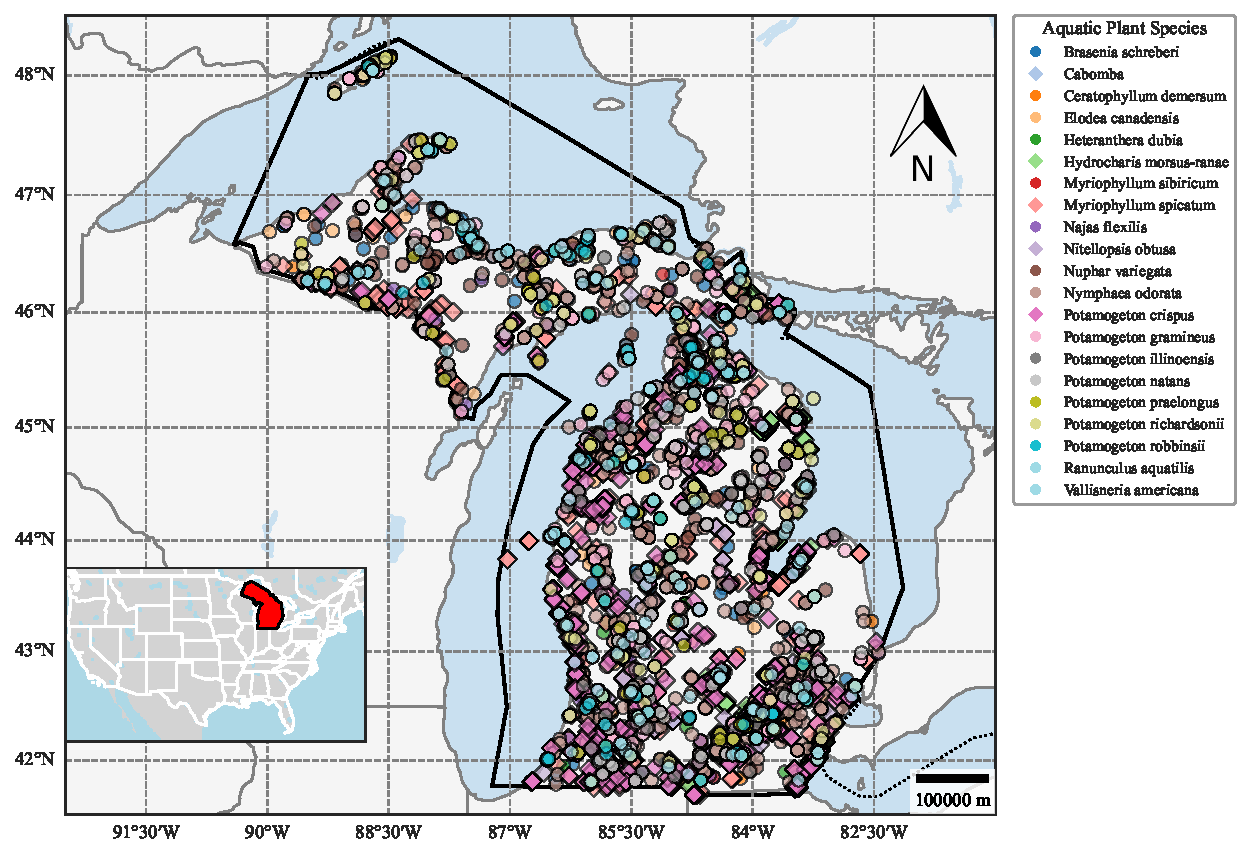
\includegraphics[width=1.0\textwidth]{figs/map.pdf}
\caption{Map of Michigan illustrating the geographic focus of the study. The approximate occurrences of 21 aquatic plant species are plotted based on data from the Global Biodiversity Information Facility (GBIF). The five invasive species are denoted by diamond markers, while the 16 native species are denoted by circular markers. The inset map (bottom left) indicates Michigan's location within the contiguous United States.} 
\label{fig:map}
\end{figure*}

\subsection{Dataset details}
Data collection in underwater environments is a recognized challenge. Consequently, this study utilizes images of aquatic plants captured in a controlled laboratory setting to train the model. To evaluate generalization to unseen conditions and mitigate overfitting, an additional out-of-distribution dataset consisting of crowd-sourced images of hand-held plants was employed.

\subsubsection{Data preparation and distribution}
\begin{figure*}[!ht]
\centering
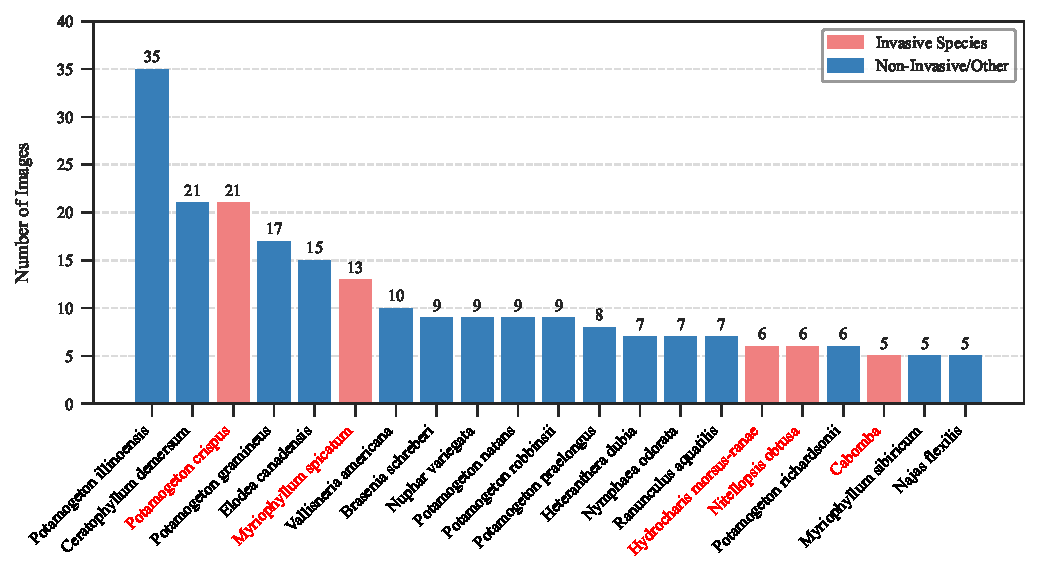
\includegraphics[width=1.0\textwidth]{figs/data_dist.pdf}
\caption{Bar plot of the distribution of the dataset with images of the aquatic plants in lab settings. It shows the number of high-resolution images available across 21 different plant species, of which 5 are invasive (denoted in red).} 
\label{fig:data_dist}
\end{figure*}

The laboratory dataset comprises a total of 230 images across 21 different plant species, 5 of which are invasive. This dataset was split into three partitions for training, validation, and testing. Stratified sampling was used to ensure a proportional distribution of all classes across the partitions. Sixty percent of the images were allocated to the training partition, with 20\% reserved for validation and 20\% for testing. This resulted in 138 images for training, and 46 images each for validation and testing. Figure \ref{fig:data_dist} shows the distribution of these images in descending order. All classes were retained, including those with only a single training instance.

The out-of-distribution dataset consisted of 33 crowd-sourced images spanning 10 of the plant species. These images were divided equally between validation and testing sets. Incorporating an out-of-distribution validation set was essential to monitor generalization and prevent the model from overfitting to the laboratory environment.

\subsubsection{Preprocessing and Augmentation}

\begin{figure*}[!h]
\centering
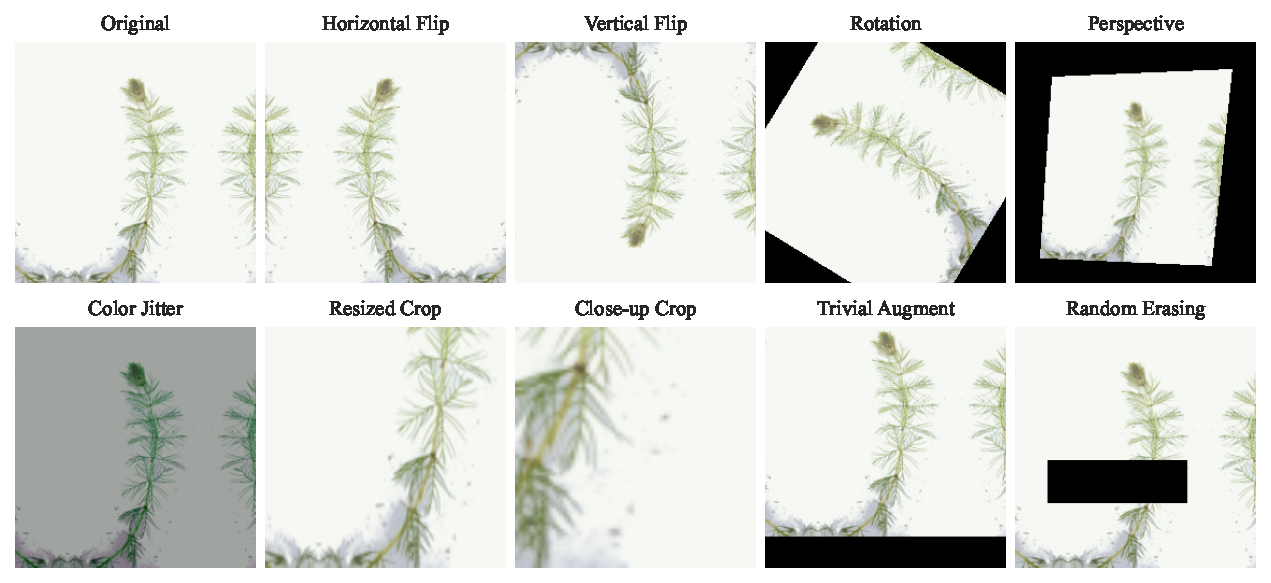
\includegraphics[width=0.9\textwidth]{figs/augmentations.pdf}
\caption{Various data augmentation techniques applied to the original images. The first row demonstrates basic geometric augmentations. The augmentations in the second row were specifically tuned to improve generalization from a small dataset. The close-up crop allows the model to learn from high-resolution details that would otherwise be lost during downsampling.} 
\label{fig:augmentations}
\end{figure*}

Basic preprocessing was conducted to remove reference artifacts, such as coins and scales, commonly present in laboratory photographs. Given the limited training set of 138 images, a comprehensive data augmentation pipeline, illustrated in Figure \ref{fig:augmentations}, was critical.

The laboratory images were captured at high resolutions (3000x4000 pixels), whereas standard pretrained convolutional backbones are optimized for smaller input dimensions (e.g., 224x224 pixels) to limit parameter count and prevent overfitting. Downsampling the original images directly to these dimensions would result in the loss of fine botanical details. To preserve these details and fully utilize the high-resolution data, the model was trained on randomly cropped patches extracted from the original images. These patches, ranging from 20\% to 100\% of the original image area, were subsequently resized to 224x224 pixels. This approach preserves high-resolution features and induces scale invariance, preparing the model for downstream resolution-dependent modules.

Following the random crop, a series of geometric transformations, including rotations, flips, and affine transformations, were applied to simulate varied camera perspectives. Natural color, brightness, and lighting variations were also introduced. These transformations were applied with a probability of 0.5 using the Torchvision library. 

The final augmentation stage involved random erasing, which masks a random rectangular region of the image. This technique prevents the model from relying on specific localized features, thereby encouraging the learning of more robust and generalized plant characteristics. Finally, the augmented images were normalized and converted to tensors prior to model training.

% \subsection{Plant Species Classification Method}

% \begin{figure}[!h]
% \centering
% 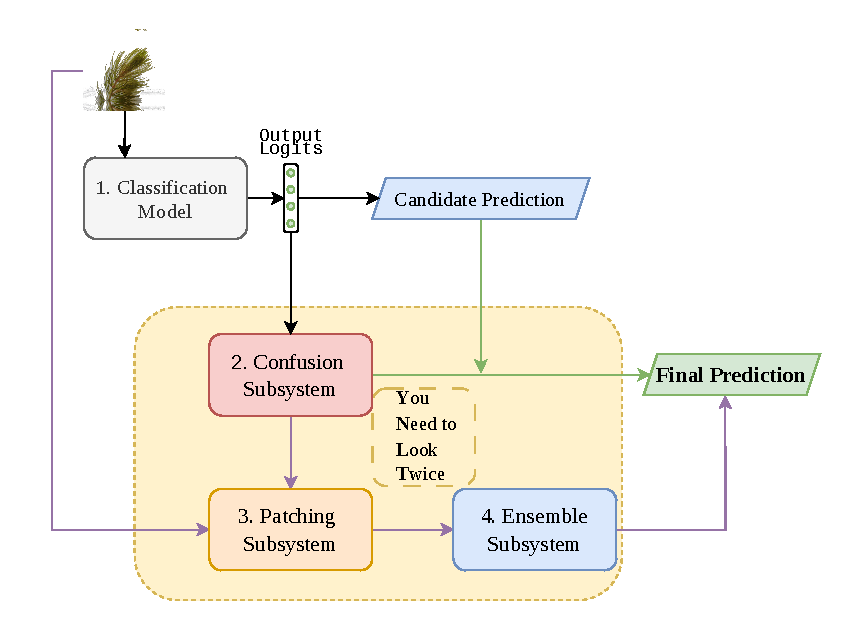
\includegraphics[width=0.5\textwidth]{figs/figs26/SimpleBlocksUpdated.drawio.pdf}
% \caption{Block diagram of the proposed Plant Species Classification Model. The image is first passed to the classification model, which outputs logits corresponding to each plant species. Based on this output, a candidate prediction as well as a corresponding evaluation of how confused the model is, is carried out. If the model is not confused, then the candidate prediction is finalized. Otherwise the Patching subsystem creates patches and passes them onto the ensemble subsystem, which makes the final prediction after a closer look.} 
% \label{fig:model_block}
% \end{figure}

% % \begin{figure*}[!h]
% % \centering
% % 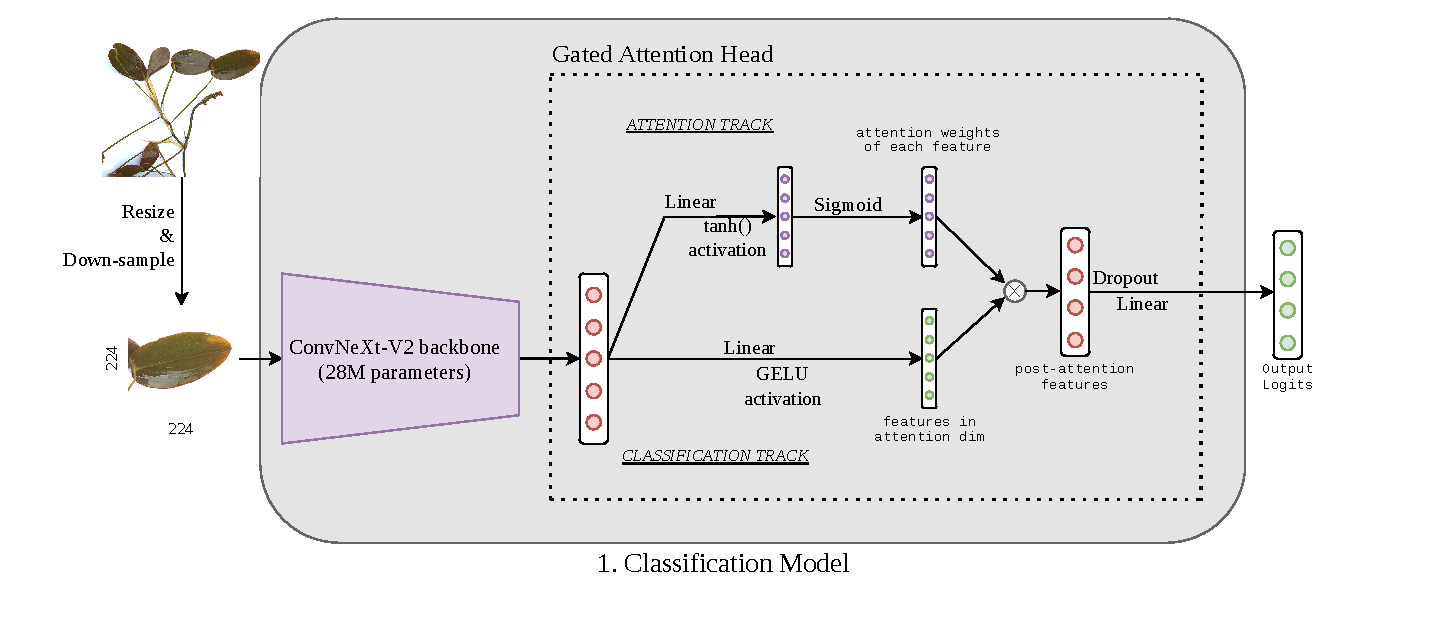
\includegraphics[width=1.0\textwidth]{figs/figs26/PlantClassification26.drawio.pdf}
% % \caption{The first stage in our proposed solution is a classification model. The input image is resized and fed to a pretrained ConvNeXt-v2 backbone for feature extraction. The output of the pretrained model is passed on to a our Gated-Attention classification head. This module has 2 parallel tracks - one for the classification features and another to compute the attention weights of those features. The outputs of both of these tracks are multiplied and the last layer outputs logits corresponding to each plant species.} 
% % \label{fig:model_block}
% % \end{figure*}


% % \begin{figure*}[!h]
% % \centering
% % 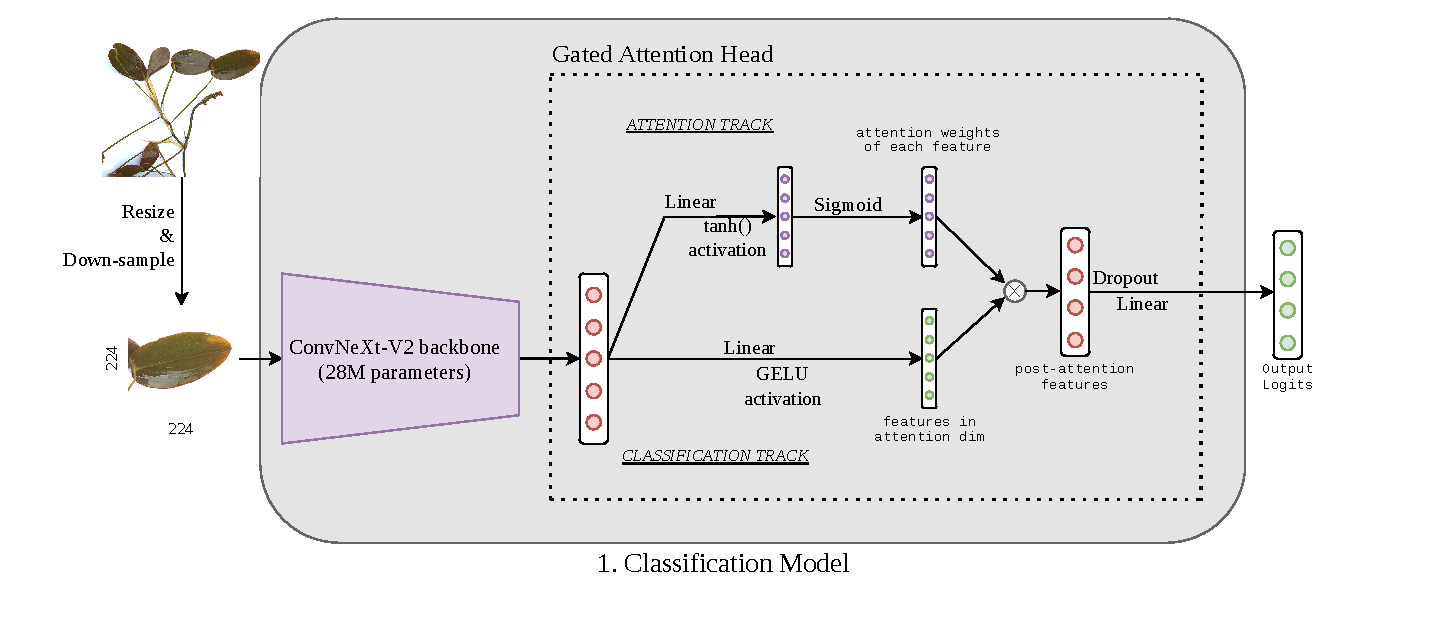
\includegraphics[width=1.0\textwidth]{figs/figs26/PlantClassification26.drawio.pdf}
% % \caption{The first stage in our proposed solution is a classification model. The input image is resized and fed to a pretrained ConvNeXt-v2 backbone for feature extraction. The output of the pretrained model is passed on to a our Gated-Attention classification head. This module has 2 parallel tracks - one for the classification features and another to compute the attention weights of those features. The outputs of both of these tracks are multiplied and the last layer outputs logits corresponding to each plant species.} 
% % \label{fig:model_block}
% % \end{figure*}


% \begin{figure*}[!h]
% \centering
% 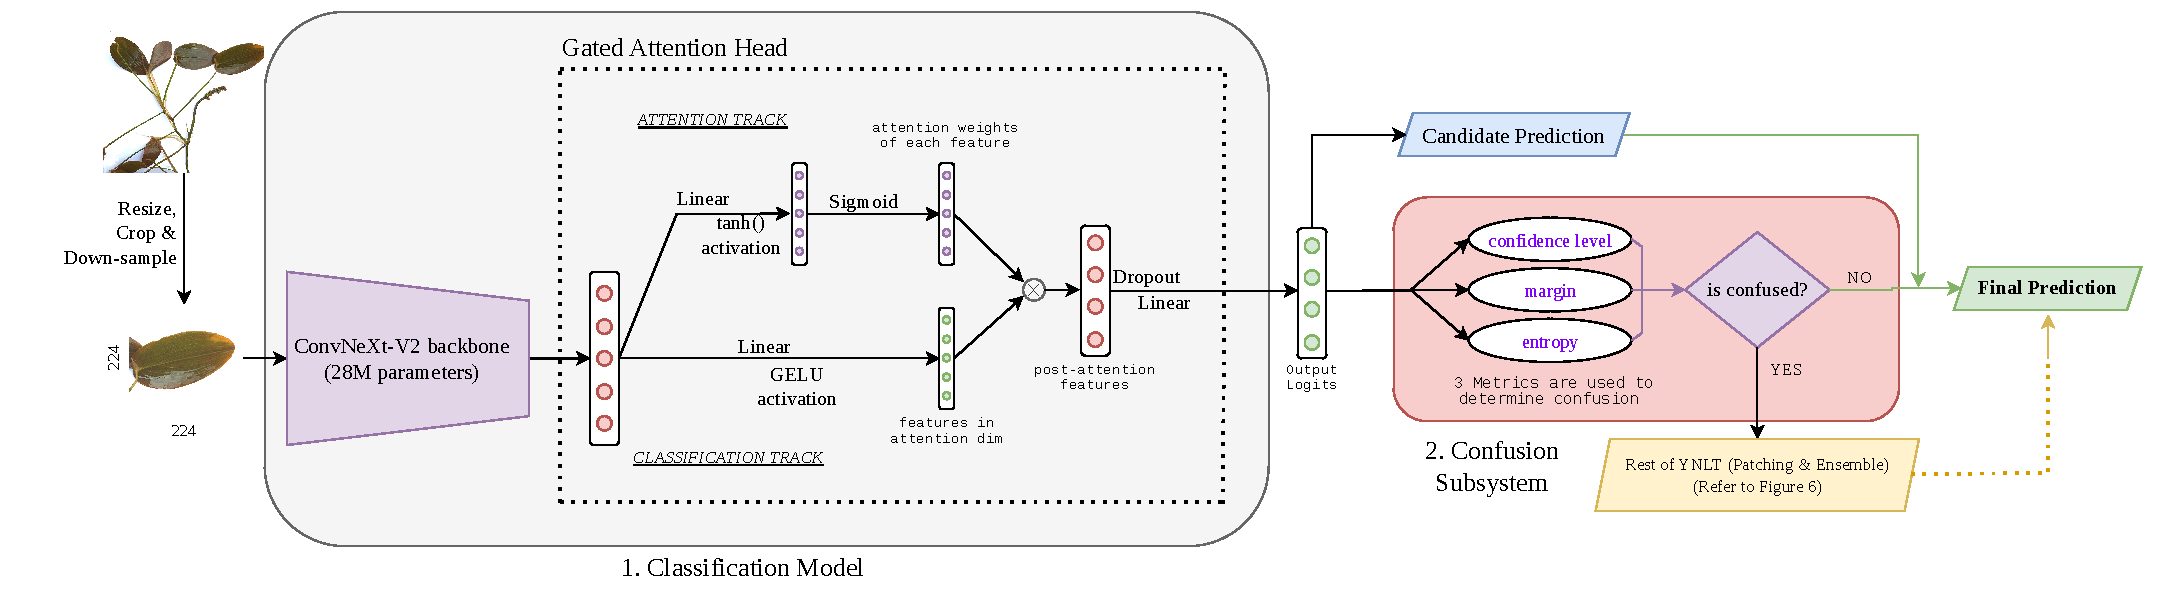
\includegraphics[width=1.0\textwidth]{figs/figs26/CombinedClassificatioAndConfusion.drawio.pdf}
% \caption{First 2 Modules} 
% \label{fig:model_block}
% \end{figure*}

\subsection{Plant Species Classification Method}

\begin{figure*}[!h]
\centering
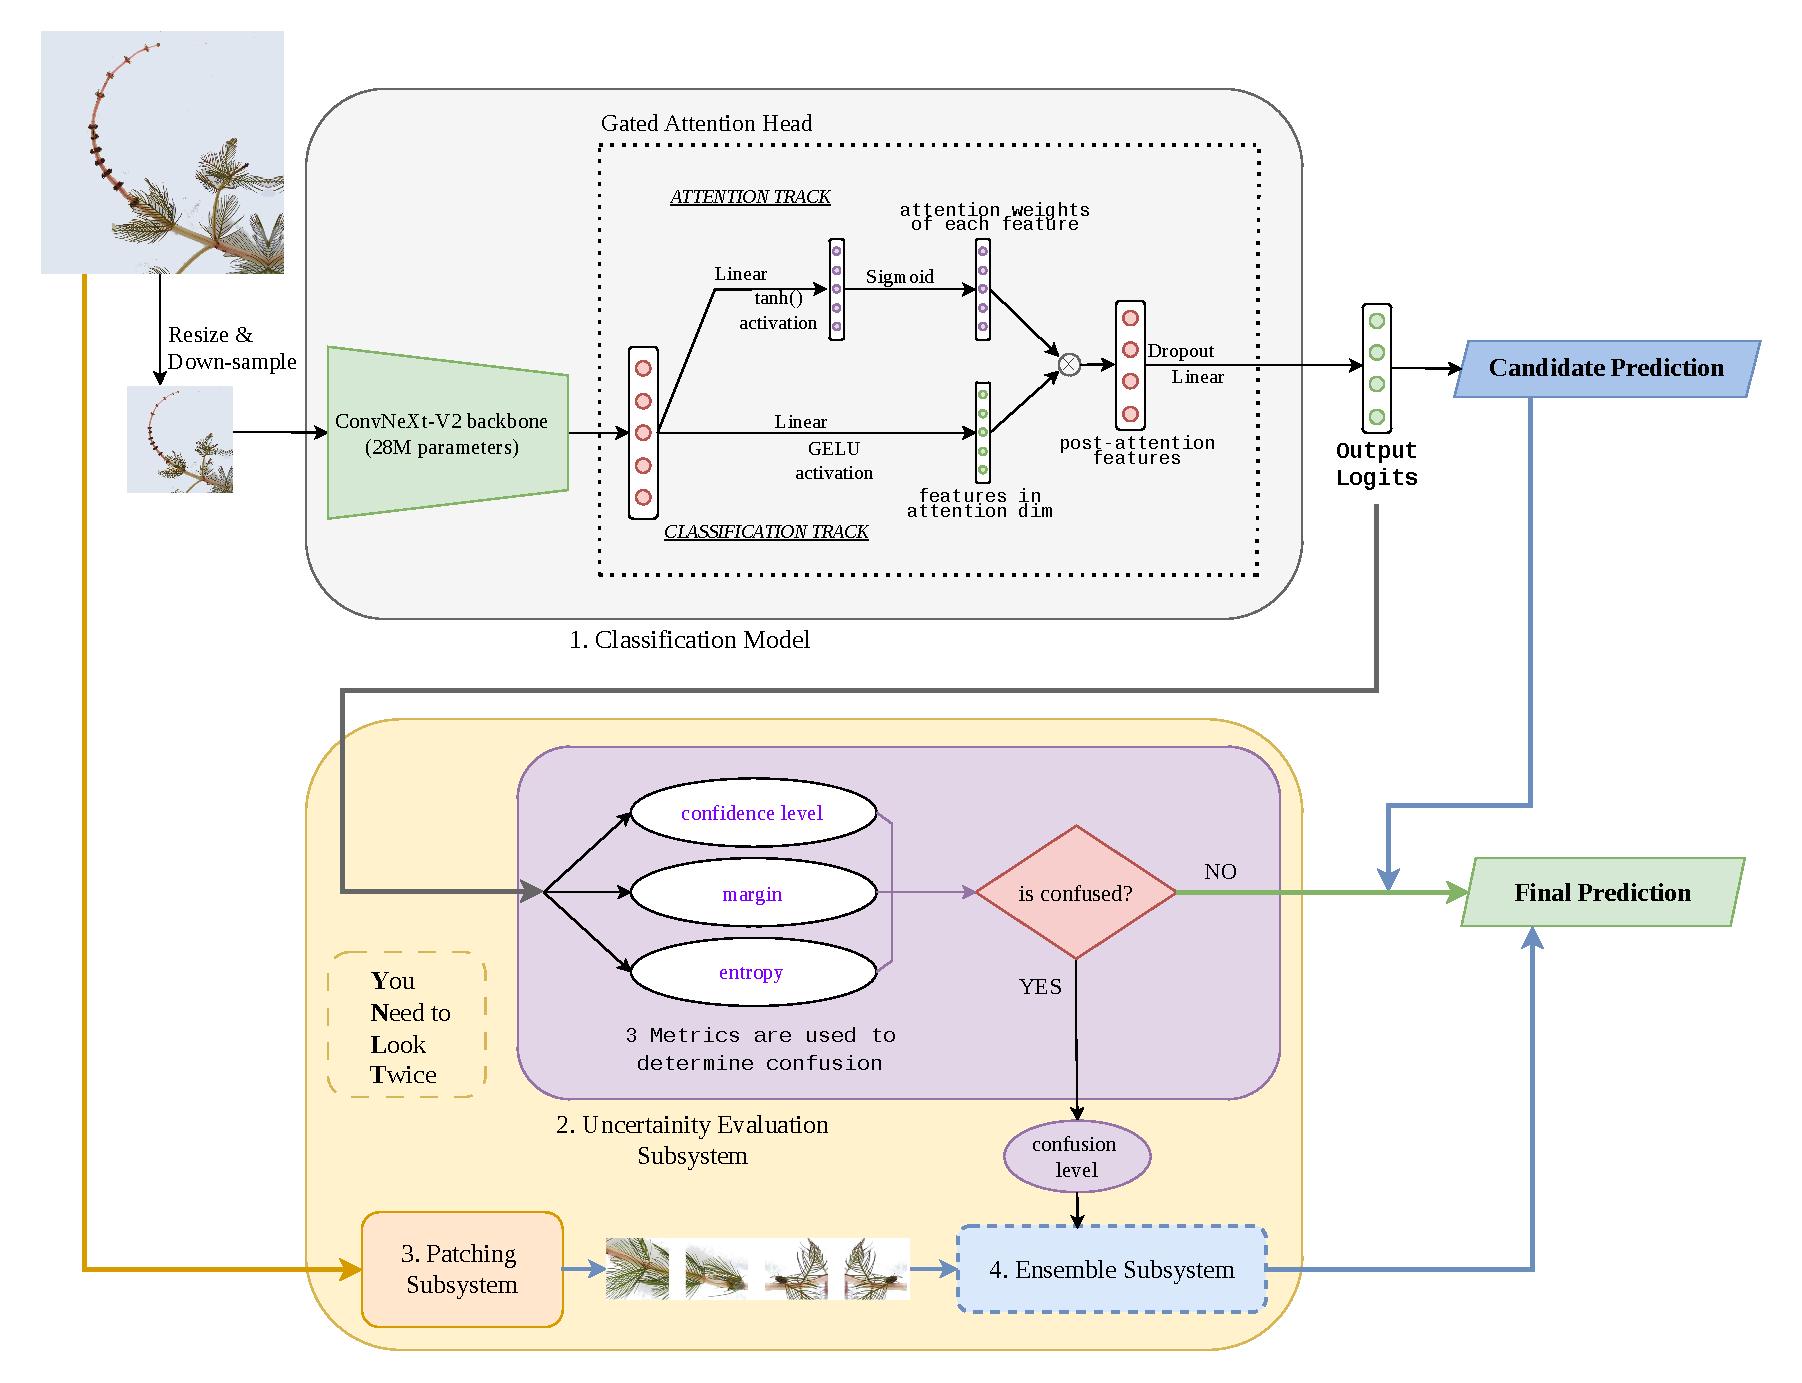
\includegraphics[width=1.0\textwidth]{figs/figs26/CombinedClassificatioAndConfusion_simplified.drawio.pdf}
\caption{Block diagram of the proposed Plant Species Classification pipeline. The system consists of two primary modules: (1) a feature extraction and classification network that outputs initial class logits, and (2) an uncertainty evaluation and ensembling system (YNLT) that assesses prediction confidence and re-evaluates the image using high-resolution patches if necessary.} 
\label{fig:model_block}
\end{figure*}

As illustrated in Figure \ref{fig:model_block}, the proposed architecture consists of two primary pathways. The first is the classification module, which processes an input image or patch to generate class-specific logits. The second module is the uncertainty evaluation system, which assesses the confidence of the initial prediction and, if necessary, triggers a high-resolution re-examination to finalize the classification.

\subsubsection{Pretrained ConvNeXt-V2 Backbone}

ConvNeXt-V2 integrates modern architectural advancements inspired by transformer models into a convolutional framework \cite{Wooetal2023}. It incorporates mechanisms such as larger convolutional kernels and global response normalization (GRN) while retaining the spatial inductive biases characteristic of standard convolutional operations. This architecture provides high representational capacity without introducing the excessive parameter count typically associated with pure transformer models. Parameter efficiency is particularly critical for this study, as the limited training dataset significantly increases the risk of overfitting.

A primary advantage of utilizing ConvNeXt-V2 for this specific problem is its rigorous pretraining methodology. The model was pretrained using a Fully Convolutional Masked Autoencoder (FCMAE) framework \cite{Wooetal2023}, followed by supervised training on ImageNet-22k and final fine-tuning on ImageNet-1k. The ImageNet-22k dataset encompasses a vast hierarchical class structure, including several aquatic plant species within the same taxonomic families as those in the target dataset, such as pondweeds and waterlilies. Consequently, the pretrained backbone acts as a highly effective feature extractor, having already learned relevant morphological representations of aquatic flora prior to fine-tuning on the laboratory dataset.

\subsubsection{Gated Attention Classification Head}

The ConvNeXt-V2 backbone extracts a global feature vector of length 768. While a standard linear classifier could map these features directly to the target plant species, it lacks the capacity to suppress irrelevant environmental artifacts encoded within the vector. Conversely, integrating a standard multi-head self-attention module would introduce an excessive number of trainable parameters, severely increasing the risk of overfitting on the limited laboratory dataset.

To resolve this architectural trade-off, a parameter-efficient Gated Attention classification head was implemented, drawing inspiration from Gated Linear Units (GLUs) \cite{Dauphinetal2017} and query-dependent gating mechanisms \cite{Qiuetal2025}. This module utilizes a dual-branch architecture: a standard feature projection pathway (a Multilayer Perceptron) and a parallel attention branch designed to learn the relative importance of each feature. After applying a GELU activation function \cite{HendrycksandGimpel2016}, the learned attention weights are multiplied element-wise with the projected features to generate the final class logits.
\subsection{You Need To Look Twice (YNLT) Module}

The design of the YNLT module is based on a common human response: taking a closer look when unsure. If analyzing the full image does not result in a confident prediction, the system extracts and examines smaller, high-resolution patches. This approach is highly relevant for aquatic plant identification. Many native and invasive species look very similar from a distance and can only be told apart by looking at fine physical details.

\subsubsection{Uncertainty Evaluation Subsystem}

To quantify the model's predictive uncertainty—a critical component for reliable decision-making under distributional shift \cite{Ovadiaetal2019}—three metrics are derived from the output logits of the Gated Attention head: Confidence, Margin, and Entropy. Relying solely on the maximum softmax probability (Confidence) is often insufficient, as modern high-capacity neural networks are notoriously prone to overconfident misclassifications \cite{Guoetal2017}. To capture a more holistic measure of ambiguity, Margin is defined as the difference in probability between the most likely and the second most likely classes. Entropy quantifies the overall dispersion of the probability distribution and is calculated as:

To quantify the model's uncertainty, three metrics are derived from the output logits of the Gated Attention head: Confidence, Margin, and Entropy. Confidence represents the maximum softmax probability assigned to the predicted class. Margin is defined as the difference in probability between the most likely and the second most likely classes. Entropy quantifies the overall dispersion of the probability distribution and is calculated as:

\[
H(X) = -\sum_{i=1}^n p_i \log_2 p_i
\]
where \( p_i \) is the predicted probability associated with class \( i \), and \( n \) is the total number of classes.

Based on these three metrics, the initial prediction is assigned an uncertainty coefficient \( c_i \), defined strictly as:

\[
c_i \in \{0, 1, 2, 3\}
\]

where 0 indicates high certainty and 3 indicates severe ambiguity. If the uncertainty coefficient \( c_i \) exceeds a pre-configured threshold, the initial candidate prediction is suspended, and the image is passed to the patching subsystem for high-resolution re-evaluation.

\subsubsection{High-Resolution Patching Subsystem}

When a prediction is flagged for high uncertainty, it indicates that the downsampled 224x224 input image lacks the fine morphological details necessary for accurate classification. To resolve this, the patching subsystem systematically extracts multiple overlapping patches at various scales directly from the original high-resolution image. The patching parameters, including scale and overlap, are configurable to balance accuracy and computational efficiency. Processing a higher number of intermediate scales with greater overlap captures more localized detail, which can improve accuracy at the cost of increased inference time. Once generated, all extracted patches are forwarded to the ensemble subsystem to determine the final prediction.

\subsubsection{Ensemble Subsystem}

The Ensemble subsystem executes the actual ``second look" within the YNLT framework. It receives the collection of localized, high-resolution patches generated by the preceding subsystem and evaluates them to resolve the initial visual ambiguity. By shifting the model's focus from the downsampled global image to these detailed morphological features, the system gathers the precise evidence needed to make an informed final classification.

\begin{figure*}[!h]
  \centering
  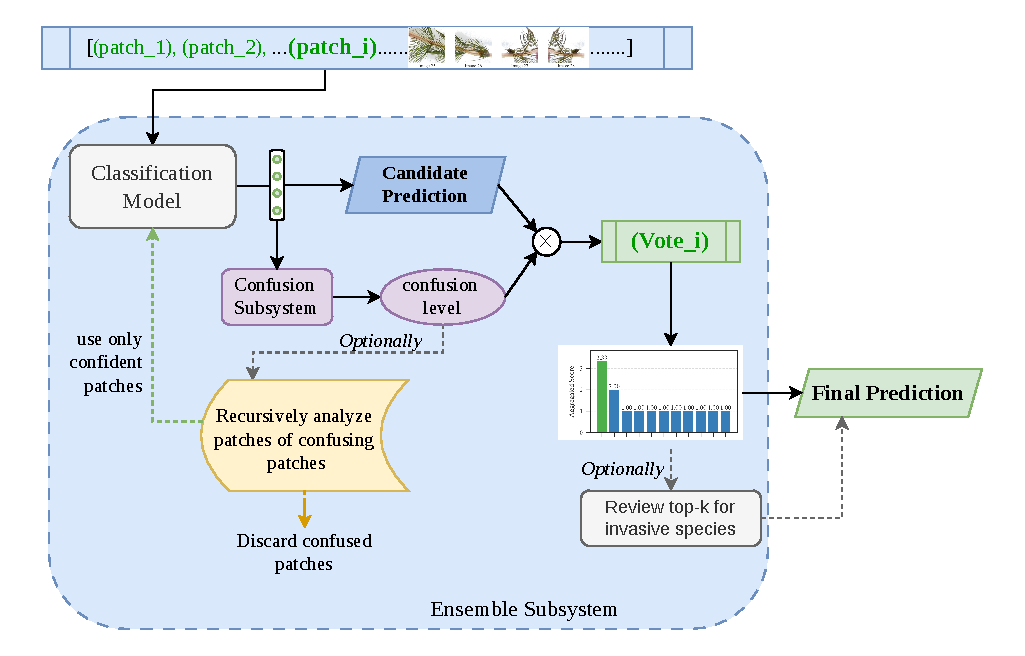
\includegraphics[width=1.0\textwidth]{figs/figs26/ensemble26_simplified.drawio.pdf}
  \caption{Workflow of the Ensemble subsystem. An image flagged for high uncertainty is divided into high-resolution patches. Each patch is processed independently by the classification pipeline and contributes a weighted vote to the final aggregated prediction.}
  \label{fig:ensemble}
\end{figure*}


Each generated patch is processed independently by the classification module. The model maintains robust performance on these localized inputs due to the scale-invariant representations learned during the data augmentation phase. Because not all patches contain identifiable botanical features, each patch generates both a candidate prediction and a corresponding uncertainty coefficient. 

The final classification is determined through an ensemble voting mechanism. To ensure that highly ambiguous patches do not disproportionately influence the outcome, each patch's vote is weighted inversely to its uncertainty. The weight \( W_i \) for a given patch prediction is calculated as:

\[
W_i = 4 - c_i
\]
where \( c_i \in \{0, 1, 2, 3\} \) is the calculated uncertainty coefficient for that specific patch.

To further minimize the False Negative Rate for critical classes, the subsystem incorporates a risk-averse thresholding strategy. If an invasive species appears within the top-\(k\) aggregated predictions of the ensemble, the system defaults to the invasive classification. This mechanism ensures that the ecological risks associated with overlooking an aquatic invasive species are systematically mitigated.

\subsection{Evaluation Metrics}

During training, the primary indicators used to monitor model convergence were validation accuracy and loss. To prevent the network from generating overconfident predictions, which would compromise the YNLT module's ability to accurately detect uncertainty, label smoothing was applied in conjunction with standard cross-entropy. As demonstrated by \citet{Mulleretal2019}, label smoothing not only improves generalization but also significantly aids in model calibration by preventing the network from assigning full probability to the target class, thereby keeping the logits constrained. The smoothed cross-entropy loss is defined as:

\[
\mathcal{L}_{\text{smooth}} = - \sum_{i=1}^{K} q_i \log p_i
\]
where \( p_i \) is the predicted probability corresponding to class \( i \), \( K \) is the total number of classes, and the smoothed target distribution \( q_i \) is calculated as:

\[
 q_i = (1 - \epsilon) \delta_{i,y} + \frac{\epsilon}{K} 
\]
with \( \epsilon \) representing the label-smoothing factor. This regularization ensures the model produces well-calibrated probability distributions \cite{Guoetal2017, Mulleretal2019}, allowing the downstream uncertainty thresholds in the YNLT module to function reliably.

Overall model performance was evaluated using standard multi-class metrics, including overall accuracy and class-wise recall. However, given the ecological context of the study, predictions were also aggregated into a binary classification: Invasive (positive class) versus Native (negative class). In this binary framework, the most critical evaluation metric is the False Negative Rate (FNR). The ecological consequences of failing to identify an invasive species (a false negative) severely outweigh the operational costs of misclassifying a native plant as invasive (a false positive). Therefore, minimizing the FNR was a primary objective:
\[
\text{FNR} = \frac{\text{FN}}{\text{TP} + \text{FN}}
\]
where FN represents False Negatives and TP represents True Positives.

To specifically isolate and evaluate the utility of the proposed YNLT block, model predictions were tracked before and after the ensemble process. For any image flagged for high-resolution re-evaluation due to high uncertainty, there are four possible transition outcomes, as outlined in Table \ref{tab:ynlt_outcomes}.

\begin{table}[h]
    \centering
    \begin{tabular}{lcc}
        \hline
        \textbf{Case} & \textbf{Before YNLT} & \textbf{After YNLT} \\
        \hline
        1 & Correct & Correct \\
        2 & Correct & Incorrect \\
        3 & Incorrect & Correct \\
        4 & Incorrect & Incorrect \\
        \hline
    \end{tabular}
    \caption{Possible transition outcomes for images processed by the YNLT ensemble module.}
    \label{tab:ynlt_outcomes}
\end{table}

Based on these transition cases, two custom metrics—Success Rate and Effectiveness—were defined to quantify the module's performance:

\[
\text{Success Rate} = \frac{\text{Total Correct After YNLT}}{\text{Total Images Reviewed by YNLT}}
\]

\[
\text{Effectiveness} = \frac{\text{Transitions from Incorrect to Correct}}{\text{Total Images Reviewed by YNLT}}
\]

These metrics served as key optimization targets for tuning the uncertainty thresholds, as well as the scale and overlap parameters within the patching subsystem.

\subsection{Experimentation}
This section discusses the hyperparameters tuned and some of the design choices that were made in this work 
\subsubsection{Training Classification model}
% learning rate schedule
% AdamW optimizer
% label smoothing
The model was implemented with the PyTorch framework, on a CUDA-enabled laptop with an NVIDIA A500 laptop GPU (4 GB VRAM, 16 GB RAM). Although limited, the computational capabilities were sufficient for the small dataset used in the study. We limited the model development to only training the classification heads, leaving all the weights of the pretrained model frozen. 

The training used the AdamW optimizer, and followed a cosine-based learning rate schedule for 100 to 300 epochs with an early stopping patience ranging from 20 - 50 epochs. We also used a label smoothing factor ranging from 0.05 to 0.1

\subsubsection{Tuning YNLT Block}
% patching - scales and overlaps
% we disabled recursion - may set a max depth
The YNLT block is designed to be configurable. There is a trade-off between efficiency and effectiveness. One can set a list of different scales and corresponding overlaps for the patching subsystem to extract patches from images that the model finds confusing. While more scales and overlaps make this block more effective, it also causes the final prediction to take longer. 

Alternatively, one can also allow the block to recursively look at finer details in the image, instead of setting very small scales to begin with. To prevent infinite recursion, one must also set a max-depth for the recursion to stop at.


%%%%%%%%%%%%%%%%%%%%%%%%%%%%%%%%%%%%%%%%%%%%%%%%%%%%%%%%%%%%
% \begin{table*}[!ht]
% \caption{Summary of YOLO variants with open-source software packages.}
% \label{tab:models}
% \renewcommand{\arraystretch}{1.4}
% \centering
% \resizebox{0.7\textwidth}{!}{
% \begin{tabular}{llll}
% \hline
% Index & YOLO models  & URL & Reference \\ \hline
% 1     & YOLOv3    & \url{https://github.com/ultralytics/YOLOv3}  & \cite{redmon2018YOLOv3}         \\ 
% 2     & YOLOv4    & \url{https://github.com/WongKinYiu/PyTorch-YOLOv4}  & \cite{bochkovskiy2020YOLOv4} \\ 
% 3    & YOLOv5   & \url{https://github.com/ultralytics/YOLOv5}   & \cite{jocher2020YOLOv5}           \\
% 4   & Scaled-YOLOv4     & \url{https://github.com/WongKinYiu/ScaledYOLOv4}   & \cite{wang2021scaled}           \\ 
% 5    & YOLOR      & \url{https://github.com/WongKinYiu/yolor} & \cite{wang2021r}           \\ \hline
% \end{tabular}
% }
% \end{table*}





%%%%%%%%%%%%%%%%%%%%%%%%%%%%%%%%%%%%%%%%%%%%%%%%%%%%%%%%%%%%

\section{Results}
\label{sec:results}


\begin{table*}[!ht]
    \caption{Ablation experiments to measure contribution of different components of the proposed solution to improving results on the lab and out-of-distribution test sets. The last row represents our proposed solution with both the novel components (Gated Attention and the YNLT block). All the model configurations use the same pretrained ConvNeXt-V2 backbone for feature extraction.}
    \label{tab:ablation}
    \renewcommand{\arraystretch}{1.4}
    \centering
    \resizebox{1.0\textwidth}{!}{
         \begin{tabular}{lcccccc}
             \hline
             \multirow{2}{*}{\textbf{Model}} & \multicolumn{3}{c}{\textbf{Lab Data (\%)}} & \multicolumn{3}{c}{\textbf{OOD Data (\%)}} \\
             \cline{2-4} \cline{5-7}
             & \textbf{Class Acc} & \textbf{Bin Acc} & \textbf{Bin FNR} & \textbf{Class Acc} & \textbf{Bin Acc} & \textbf{Bin FNR} \\
             \hline
             Linear Classifier & 84.78 & 93.48 & 30.0 & 47.06 & 58.82 & 62.5 \\
             Linear + YNLT Block & 91.30 & 93.48 & 30.0 & 52.94 & 58.82 & 62.5 \\
             Gated Attention Classifier & 86.96 & 97.83 & 10.0 & 52.94 & 76.47 & 12.5 \\
             Gated Attention + YNLT Block & 93.48 & 97.83 & 10.0 & 64.71 & 76.47 & 12.5 \\
             \hline
        \end{tabular}
    }
\end{table*}

\subsection{Ablation Tests}
The study included ablation tests to measure the contribution of different components of our proposed solution towards improving the results. The proposed solution has 3 main components - (1) the ConvNeXt-v2 backbone for feature extraction, (2) the Gated Attention head for classification, and (3) the YNLT block to take a second look and ensemble predictions from higher-resolution patches.

From the second entry of Table \ref{tab:ablation} it can be seen that using a Gated Attention based classifier significantly improves performance over a simple linear classifier from 84.78\% to 86.96\%. These results are with a Gated Attention head with an attention dimension set to 168, resulting in 261,933 trainable parameters. This is more efficient and appropriate for small datasets to mitigate the risk of overfitting. Performance may further improve with higher parameter counts, given more training images. 

The last entry of the Table \ref{tab:ablation} enumerates the performance of the final proposed solution with the Gated Attention head and the YNLT block, which complement each other. This combination also generalizes better, and has a significantly higher accuracy on the out-of-distribution data at 64.71\%.

From the above, it can be seen that all components of the proposed solution contribute to increasing the performance metrics. And they also complement each other, as the gain in performance from using both of them together is higher than the sum of their contributions separately.

%TODO:
% 1. Also talk about FNR decrease
% 2. Include final \% numbers in the above

% \subsection{McMilan's Test}

\subsection{Best Model Performance}

The last row in Table \ref{tab:ablation} shows that the best performing model is a combination of a Gated Attention based classification head on a ConvNeXt-V2 backbone for feature extraction, along with the proposed YNLT block. In this section we will look at the performance of this model in detail.

% Example - Figure 1 - Image and classification scores
\begin{figure*}[!h]
  \centering
  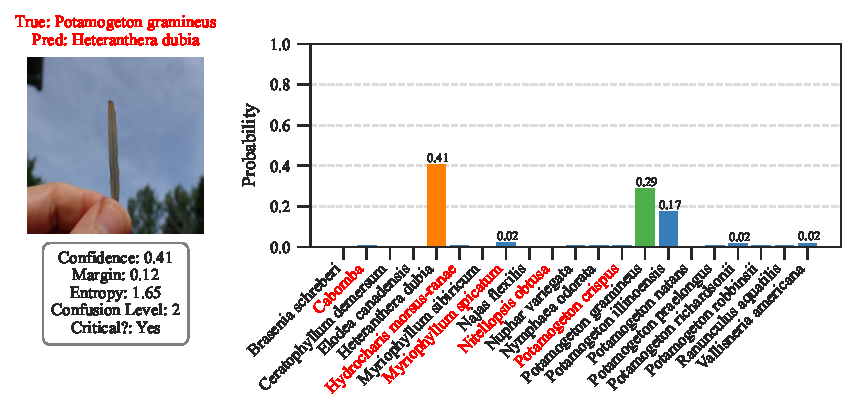
\includegraphics[width=1.0\textwidth]{figs/sample_prediction_initial.pdf}
  \caption{Example of an initially misclassified image. The bar chart shows the model’s output probabilities, where the highest logit corresponds to Heteranthera dubia while the true label is Potamogeton gramineus. The uncertainty metrics (bottom left) indicate model confusion and trigger the YNLT block to re-examine the image. The corrected prediction after the second pass is shown in the following figure.}
  \label{fig:incorrect}
\end{figure*}
%The figure shows a detailed report of one of the images that was initially classified incorrectly. The bar graph on the right shows the probability distribution from the output of the classification model. The highest logit corresponds to Heteranthera dubia, but the image actually is of Potamogeton gramineus. Even though the model is wrong, it accurately communicates that it is confused through the metrics listed in the box at the bottom left. This signals the YNLT block to take a second closer look at the image. In this particular example, the revised prediction after a second look was correct, as seen in the next figure.


The first component of our solution is the classification model that taken an input image and outputs logits corresponding to the probabilities of the image belonging to each of the 21 species of plants. Figure \ref{fig:incorrect} illustrates this stage with a sample image belonging to the Potamogeton gramineus species from the out-of-distribution test set. The bar graph in \ref{fig:incorrect} represents the probability distribution from the output of the classification model. We observe that the second highest predicted probability actually corresponds to the correct species. Even though this initial prediction is wrong, the model is not very confident with this prediction. The confidence is only 0.41, and the margin, which is the difference between the confidence score and that of the second highest prediction is 0.12. In this particular example, the entropy of the distribution which is also one of the metrics used to evaluate confusion is not very high. It is at moderate value of 1.65. But because two of the three metrics signal that the model is confused, the image is passed on to the YNLT block before a final prediction is made.

% Example - Image 2 - YNLT Aggregate Voting scores
\begin{figure}[!h]
  \centering
  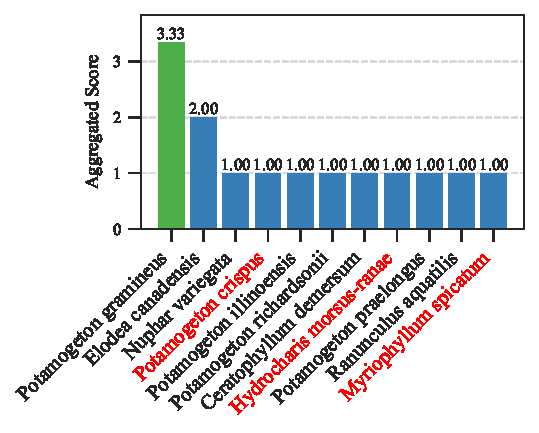
\includegraphics[width=0.48\textwidth]{figs/sample_prediction_final.pdf}
  \caption{The figure shows the aggregated scores from the voting in the Ensemble subsystem that was done for the image in the previous figure. Potamogeton gramineus is the revised final prediction with the highest votes, which in this particular example is correct.}
  \label{fig:ynlt_corrected}
\end{figure}

The second component of our solution as illustrated in \ref{fig:ensemble} first creates patches from the original high-resolution version of the current image, and then aggregates votes weighted by the confidence level of each patch. For the sample image discussed in Figure \ref{fig:incorrect}, the aggregate scores from this step are shown in Figure \ref{fig:ynlt_corrected}. The highest score corresponds to the Potamogeton gramineus species, which turns out to be the correct prediction for this image.

% Confusion matrices and classwise analysis

% \begin{figure}[!h]
%   \centering
%   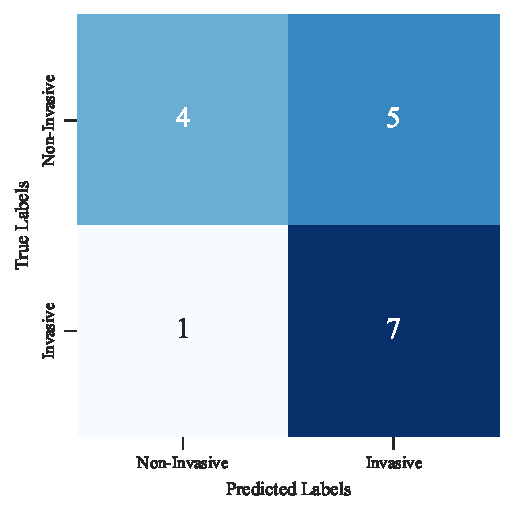
\includegraphics[width=0.45\textwidth]{figs/figs26/ood_binary_cm.pdf}
%   \caption{Binary Confusion Matrix on the out-of-distribution test set of crowd-sourced images. Binary categories were created by grouping all the native and invasive plant species together.}
%   \label{fig:bin_cm}
% \end{figure}

% \begin{figure*}[!h]
%   \centering
%   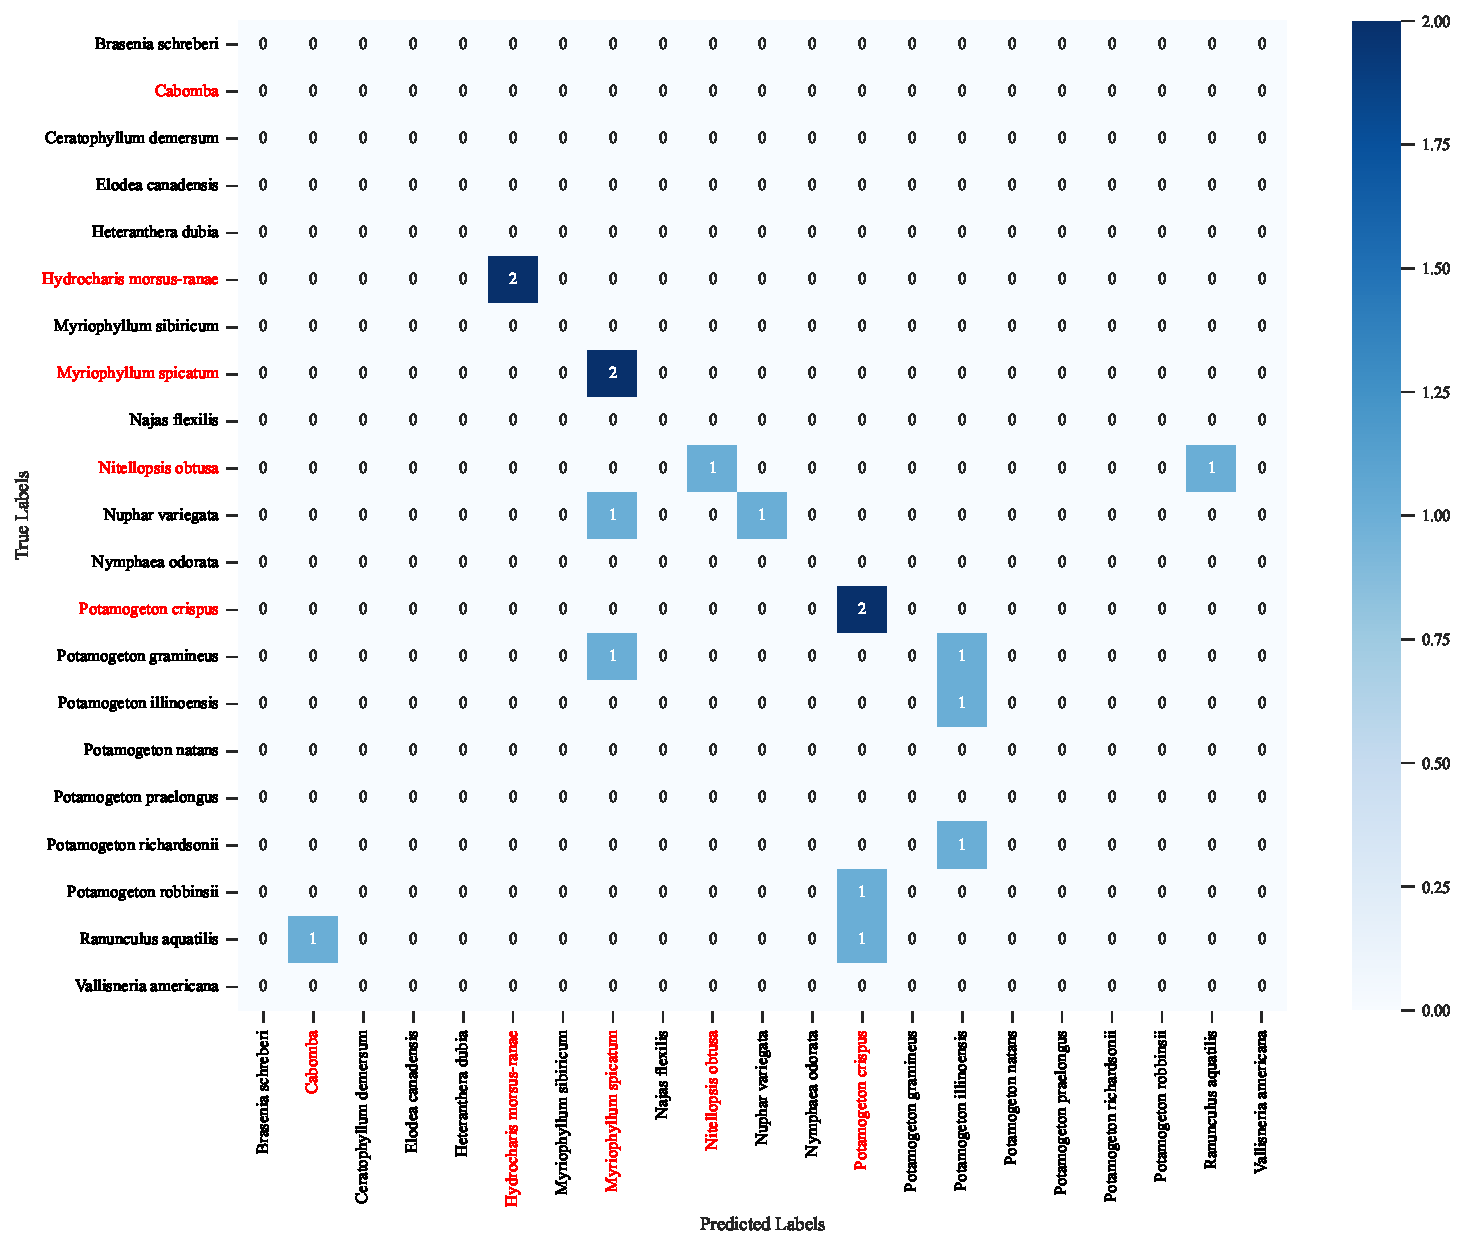
\includegraphics[width=1.0\textwidth]{figs/figs26/ood_classwise_cm.pdf}
%   \caption{The figure tabulates the classwise confusion matrix of the predictions made on the out-of-distribution test set. The numbers on the diagonal represent correct predictions. We can also see which species the model gets confused between from the non-diagonal entries.}
%   \label{fig:classwise_butterfly}
% \end{figure*}


% \begin{figure*}[!h]
%   \centering
%   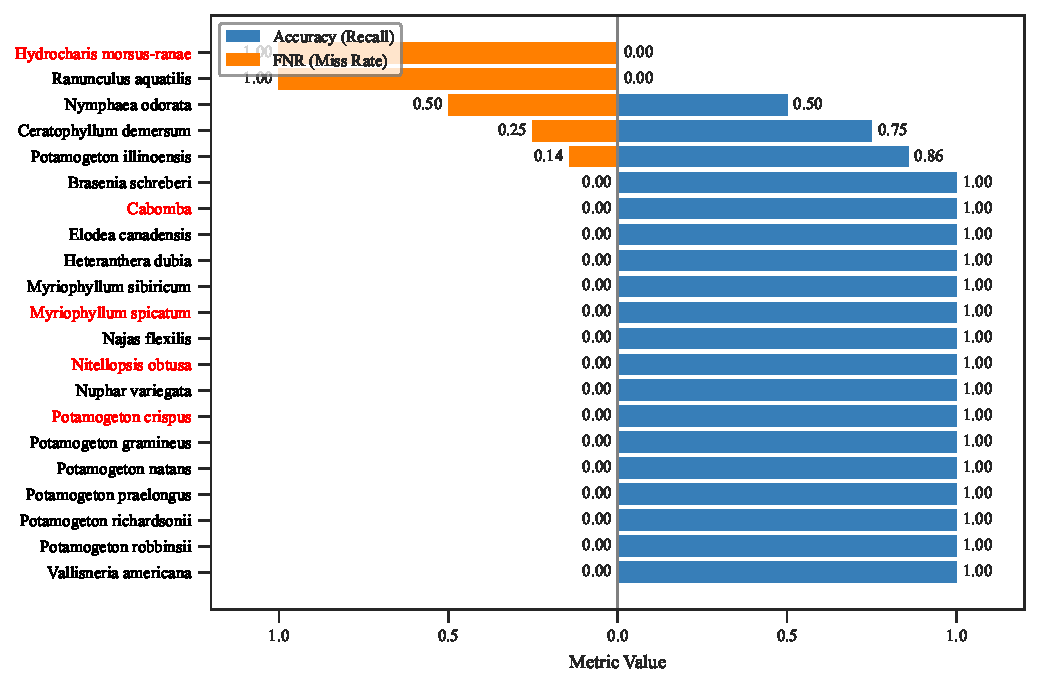
\includegraphics[width=1.0\textwidth]{figs/figs26/lab_butterfly_chart.pdf}
%   \caption{The figure is a butterfly bar graph representing classwise metrics on the best model's performance on the test set.The two metrics here are Recall or accuracy, which we are trying to maximize, and the False Negative Rate, which we aim to minimize. It can be observed that the model performs reasonably well on all classes except Hydrocharis morsus-ranae.}
%   \label{fig:classwise_butterfly}
% \end{figure*}

\section{Discussion}

\textbf{Overcoming Data Scarcity through Scale-Invariant Patching}
The primary challenge in applying deep learning to aquatic plant identification is the high cost of acquiring large, annotated datasets from underwater environments. While laboratory and crowd-sourced images are more accessible, models trained on small datasets of high-resolution images often suffer from the curse of dimensionality when downsampled to standard input sizes. This study addressed this limitation by implementing a probabilistic crop and resize augmentation strategy. By training the model on overlapping patches ranging from 20\% to 100\% of the original image size, the network learned scale-invariant representations of fine morphological details. This approach allowed the model to maximize the utility of the limited 230-image laboratory dataset without losing critical botanical features during standard downsampling.

\textbf{Architectural Suitability for Domain Generalization}
The choice of the ConvNeXt-V2 backbone and the custom Gated Attention head was critical for generalizing from controlled laboratory settings to out-of-distribution crowd-sourced images. ConvNeXt-V2 provided a parameter-efficient foundation, minimizing the risk of overfitting. Furthermore, its pretraining on ImageNet-22k included hierarchical classifications of aquatic plants such as pondweeds and waterlilies. This extensive pretraining equipped the backbone with highly relevant feature extraction capabilities before fine-tuning. However, because these extracted features also contain domain-specific background noise from the laboratory environment, the Gated Attention head was introduced. By explicitly learning to suppress background artifacts and isolate plant-specific signals, the attention mechanism enabled the model to maintain robust performance across varying environments, contributing directly to the 64.71\% accuracy achieved on the unseen crowd-sourced dataset.

\textbf{Addressing Uncertainty with the YNLT Module}
Standard downsampling often obscures the subtle visual distinctions between native and invasive aquatic species. The proposed `You Need To Look Twice' (YNLT) module resolved this by selectively extracting and ensembling high-resolution patches only when the initial prediction exhibited high uncertainty. For this mechanism to function effectively, the model's confidence scores needed strict calibration. The integration of label smoothing during training prevented the network from generating overconfident incorrect predictions, ensuring that visual ambiguity triggered the YNLT re-evaluation rather than being ignored. By dynamically shifting focus to localized, high-resolution features, the YNLT module successfully corrected ambiguous predictions and played a central role in minimizing the False Negative Rate, a critical metric for invasive species management.

\textbf{Optimization Trade-offs for Real-World Deployment}
Optimizing purely for laboratory validation accuracy often degrades performance in real-world scenarios. In this study, model selection was guided by an out-of-distribution validation set rather than relying exclusively on laboratory metrics. Training was halted when OOD validation performance plateaued, prioritizing generalizability over maximizing laboratory accuracy. This strategic trade-off proved essential, as models selected via this dual-validation method significantly outperformed lab-optimized models on the crowd-sourced test set. 

\textbf{Limitations and Future Work}
The primary limitation of this study remains the absolute size of the training dataset. While the proposed architecture effectively mitigated data scarcity, performance across all metrics is expected to scale with the introduction of more training data. Future research will explore semi-supervised or unsupervised learning techniques, such as Masked Autoencoders, to leverage large volumes of unlabeled crowd-sourced plant imagery prior to supervised fine-tuning. Additionally, future iterations will focus on model distillation. The current ConvNeXt-V2 backbone contains 28 million parameters, which is computationally expensive for edge deployment. Developing lightweight models capable of running onboard autonomous underwater vehicles, drones, or smartphones with constrained power resources will significantly expand the practical applications of this system.

\textbf{Broader Impacts}
The methodologies developed in this study offer highly scalable tools for the aquaculture, fisheries, and environmental management sectors. Deployed on mobile devices, these models can assist farmers and field workers in identifying invasive species early, minimizing both crop loss and the need for broad-spectrum chemical interventions. Furthermore, integration with autonomous robotic systems could enable continuous ecosystem monitoring and precise, targeted eradication efforts. Ultimately, accurate and efficient identification of aquatic invasive species is a foundational step in preserving native biodiversity and maintaining the economic resilience of freshwater fisheries.



%%%%%%%%%%%%%%%%%%%%%%%%%%%%%%%%%%%%%%%%%%%%%%%%%%%%%%%%%%%%%%%%%%%%%%%%%%%%%%%%%%%%%%
\section{Conclusion}
\label{sec:conclu}
% summarise work - data and main contributions
% applications and broader impact 
This study aimed to create a classification model to identify AIS, specifically in the Lakes of Michigan. A small dataset of 230 images in controlled laboratory settings were used to train a model that generalized well to images of the same plants in out-of-distribution settings such as crowd-sourced images of the plants held by people in their hands.
The main contributions of this work are as follows
\begin{enumerate}
    \item Classification model with a custom Gated Attention Head classifier to accurately identify AIS
    \item Novel YNLT Module to ensemble predictions from multiple patches of high-resolution images
\end{enumerate}

The models proposed in this study can be deployed to serve a variety of applications in domains ranging from fisheries and aquaculture to sustainable environmental management.



\section*{Authorship Contribution}

\textbf{Aaryan Panigrahi}: Formal analysis, Software, Writing - original draft; \\
\textbf{Fengying Dang}: Conceptualization, Investigation, Data curation, Supervision, Writing - original \& draft \& review \& editing.  

\section*{Acknowledgement}
The authors thank Dr. Jo Latimore for providing the weed images that supported the experimental evaluation.

% This work was supported in part by ???. 
% helping annotate the weed images and Dr. ??? for the assistance in weed identification. 

\typeout{}
% \bibliographystyle{model1-num-names}
\bibliography{ref}
\end{document}

